\section{不同空间上的映射与比较}
\label{sec:measure-cross-space}

上一节的两种测度始终生活在同一个空间里，可以直接比较同一个事件。
但在机器学习中，输入和输出往往是不同性质的对象：图片与类别、状态与动作、一句外语与一句母语。
这时要先解决“质量怎样从一个空间传到另一个空间”，才能谈比较。

本节沿三条递进的线索展开。
第一条是\emph{确定映射}：每个输入被送到唯一的输出点，输入测度由此在输出空间诱导出一个\term{推前测度}。
第二条把确定映射放宽为\term{测度核}：每个输入不再对应一个点，而是对应输出空间上的一项概率分布——这正是“随机通道”“转移概率”的抽象。
第三条保留输入与输出的配对信息，用\emph{联合测度}同时描述两边，并研究何时能从联合分布反推出条件核；最后再讨论给定跨空间成本时的最优运输。
请始终注意：输出端是否匹配、以及实现这种匹配要搬动多远，是两个不同的问题。

\subsection{\term{可测映射}的推前与密度变换}

\subsubsection{\term{推前测度}与输出积分}

\paragraph{推前的定义与质量边界}

设$T:(X,\mathcal A)\to(Y,\mathcal B)$是一个可测映射，$\mu$是输入空间上的测度。
对任意目标集合$B$，一个很自然的问题是：$T$把多少输入质量送进了$B$？
答案就是$B$的原像上的输入质量：
\[
 (T_\#\mu)(B)=\mu\bigl(T^{-1}(B)\bigr).
\]
这样定义的$T_\#\mu$称为推前测度（也叫像测度）。
可测性在这里的作用是保证$T^{-1}(B)$一定是输入端的合法可测集；记号$T^{-1}$只表示取原像，并不要求$T$可逆。

$T_\#\mu$确实是一个测度：空集的原像为空，质量为零；不相交集合的原像仍不相交，且取原像与可数并可交换，所以可数可加性从$\mu$原样传过来。
又因为$T^{-1}(Y)=X$，总质量守恒：
\[
 (T_\#\mu)(Y)=\mu(X).
\]
因此有限测度推前后仍有限，概率推前后仍是概率。
但$\sigma$有限不一定保持：实轴上无限的勒贝格测度被常值映射$T(x)=0$压到一个点上，得到总质量为$+\infty$的$\delta_0$，输出空间再也无法被有限质量集覆盖。
若多个源点映到同一目标点，该点收到的质量就是各源点权重之和。

\paragraph{输出观测在输入端的表示}

推前测度最重要的计算性质，是把“对输出的平均”翻译成“对输入的平均”。
先在指示函数$g=\mathbf 1_B$上看：
\[
 \int_Y\mathbf 1_B\,d(T_\#\mu)
 =(T_\#\mu)(B)=\mu(T^{-1}B)
 =\int_X\mathbf 1_B(Tx)\,d\mu.
\]
经简单函数和非负单调逼近，对任意非负可测$g$都有
\begin{equation}
 \int_Y g\,d(T_\#\mu)=\int_X g(Tx)\,d\mu(x),
 \label{eq:measure-pushforward-integral}
\end{equation}
即“$g$在输出端的平均，等于$g\circ T$在输入端的平均”；有符号函数在绝对可积时同样成立。
这个恒等式是后面一切核计算和矩计算的入口。

接连使用两个映射时，先送$T$再送$S$与直接送复合映射一致：
\[
 (S\circ T)_\#\mu=S_\#(T_\#\mu),
\]
因为$(S\circ T)^{-1}(C)=T^{-1}(S^{-1}(C))$。
若某个自映射$T:X\to X$恰好满足$T_\#\mu=\mu$，称它\term{保持测度}，例如抛硬币中“交换正反面”的操作；这只是质量守恒的一个特例。

\subsubsection{输出密度与质量重组}

\paragraph{回用欧氏换元计算输出密度}

推前恒等式~\eqref{eq:measure-pushforward-integral}并不要求输出有密度；只有在给定参考体积且映射足够光滑时，才能谈输出密度长什么样。
设$U,V\subseteq\mathbb R^d$是同维开集，$T:U\to V$是$C^1$微分同胚（全局一一对应、逆映射光滑），输入测度相对勒贝格体积有密度$p$。
对非负测试函数$g$，先用推前恒等式，再用多元换元：
\[
 \int_Vg(y)\,d(T_\#\mu)(y)
 =\int_U g(Tx)\,p(x)\,dx
 =\int_V g(y)\,p(T^{-1}y)\,|\det DT^{-1}(y)|\,dy.
\]
对所有$g$都成立，所以输出密度为
\[
 q(y)=p(T^{-1}y)\,|\det DT^{-1}(y)|,
\]
等价地
\[
 q(Tx)\,|\det DT(x)|=p(x).
\]
直觉是：映射在$x$附近把体积放大了$|\det DT(x)|$倍，密度就要相应缩小同样倍数，才能保持小块质量不变。
平移只平移密度$q(y)=p(y-b)$；可逆线性映射$T(x)=Ax$给出$q(y)=p(A^{-1}y)/|\det A|$；镜像等负行列式映射由绝对值处理。
多对一、降维或退化映射不满足全局微分同胚条件，不能随便选一个逆分支套公式，必须老老实实用原像把所有分支的贡献加起来。

\paragraph{合并、投影与原子输出}

即使不可逆，推前测度仍然有定义，只是输出未必有普通密度。
两个典型情形值得对比。
一是投影：若$\mathbb R^2$上有密度$p(x,y)$，$T(x,y)=x$，则目标集合$B$的原像是$B\times\mathbb R$，由Tonelli定理
\[
 (T_\#\mu)(B)=\int_B\left(\int_{\mathbb R}p(x,y)\,dy\right)dx,
\]
所以输出仍是连续分布，边缘密度是把被积掉的坐标积分掉：$q(x)=\int p(x,y)\,dy$。
二是常值映射$T(x,y)=y_0$：任何目标集合的原像不是全空间就是空集，有限输入总质量$m$被整个压成一个原子$m\delta_{y_0}$，在正维空间里相对勒贝格测度没有普通密度。
对比可见：不可逆映射既可能输出连续密度，也可能输出原子；而“一个输入只对应一个输出点”始终是确定映射的限制。
若同一个输入还要按随机性把质量分给多个输出，就需要下一小节的测度核。

\subsection{测度核与\term{测度值映射}}

\subsubsection{随输入变化的输出权重}

\paragraph{测度核的两项条件}

先用有限情形建立直觉。
设输入、输出都是有限集合，一个“随机转移规则”就是一张非负矩阵$K$：第$x$行第$y$列的数表示输入$x$把多少质量送给输出$y$，把一行中若干列加起来，就得到输入$x$送给某个输出集合的总质量。
把这个想法搬到一般空间，会遇到两个要求：固定输入时，输出端的赋值必须是一个测度（才能对集合相加）；固定输出集合时，其质量随输入的变化必须可测（才能对输入测度积分）。

\begin{definition}[测度核]
\label{def:measure-kernel}
设$(X,\mathcal A)$、$(Y,\mathcal B)$是可测空间。映射
\[
 K:X\times\mathcal B\to[0,\infty]
\]
若满足：
\begin{enumerate}
 \item 对每个$x\in X$，$K_x=K(x,\cdot)$是$(Y,\mathcal B)$上的非负测度；
 \item 对每个$B\in\mathcal B$，函数$x\mapsto K(x,B)$是$\mathcal A$可测函数，
\end{enumerate}
就称$K$为从$X$到$Y$的\term{测度核}，记作$K:X\leadsto Y$。
\end{definition}

第一条管“每个输入怎样在输出端分配质量”，第二条管“这种分配怎样随输入可测地变化”，缺一不可。
请注意这里的测度核与函数空间章里衡量相似度的正定核（kernel function）只是同名，数学对象完全不同。

一般定义不限制每个$x$送出多少总质量。
本章的运算为方便起见，额外假设存在一个与$x$无关的$M<\infty$，使
\[
 K(x,Y)\leq M\qquad\text{对所有 }x,
\]
称为统一有限质量界；逐点有限$K(x,Y)<\infty$并不等于有共同上界。
若进一步
\[
 K(x,Y)=1\qquad\text{对所有 }x,
\]
则称$K$为\term{归一化测度核}（概率核、马尔可夫核）：无论输入是什么，送出的总质量恰好为$1$。
归一化是额外条件，不写进一般核的定义。

确定映射是核的最简单特例。
对可测映射$T:X\to Y$，取
\[
 K_T(x,B)=\delta_{T(x)}(B)=\mathbf 1_B(Tx):
\]
每个输入把全部质量集中在唯一输出点$T(x)$，它是一个归一化核。
所以“推前”只是“核传递”当每行都是点质量时的特例；一般核允许输入把质量分散到多个输出，且总质量可以随输入变化。

\begin{figure*}[htbp]
\centering
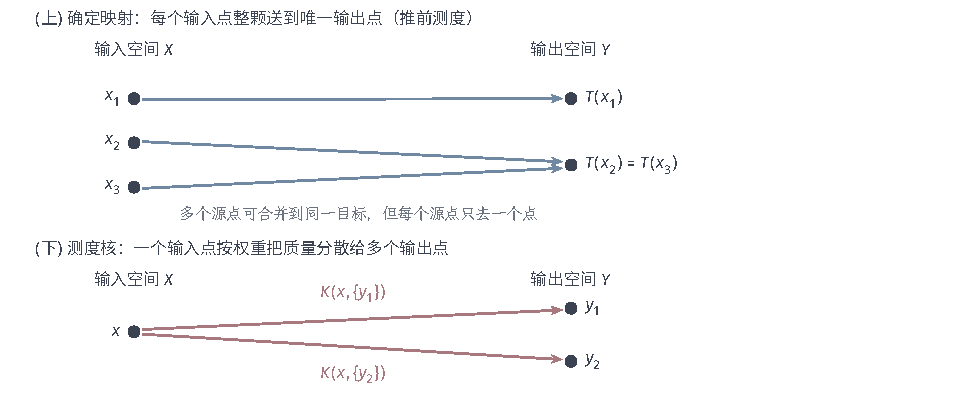
\includegraphics[width=169mm]{figures/01-mathematical-preliminaries-upper/05-space-and-geometry/tikz/pushforward-and-kernel/figure.pdf}
\caption{确定映射（推前测度）与测度核的对照。上排：每个输入点的全部质量沿唯一箭头送到一个输出点，多个输入点可以合并到同一目标（$x_2,x_3$），但单个输入点不能拆开。下排：一般测度核允许同一个输入$x$按权重$K(x,\{y_1\})$、$K(x,\{y_2\})$把质量分给多个输出；归一化核满足这些权重之和为$1$。}
\label{fig:pushforward-and-kernel}
\end{figure*}

\subsubsection{核积分与核复合}

\paragraph{输出测度与观测函数的传递}

有了输入测度$\mu$和核$K$，怎样得到输出空间上的总测度？
直观上是“每个输入$x$送出质量分布$K_x$，再按$\mu$中$x$的权重把这些分布加权求和”：
\[
 (\mu K)(B)=\int_X K(x,B)\,\mu(dx).
\]
对固定$x$，$K(x,\cdot)$可数可加；对不相交的$B_n$，用单调收敛把求和与积分交换，可知$\mu K$仍是测度。
其总质量为
\[
 (\mu K)(Y)=\int_XK(x,Y)\,d\mu\leq M\mu(X).
\]
因此统一质量界保证有限输入测度产生有限输出测度；核归一化时总质量守恒$(\mu K)(Y)=\mu(X)$，一般核则不守恒。

对应地，输出函数$g$沿核传回输入：
\[
 Kg(x)=\int_Y g(y)\,K(x,dy).
\]
对非负可测$g$，$Kg$可测，并且有核积分恒等式
\begin{equation}
 \int_Y g\,d(\mu K)=\int_X Kg\,d\mu,
 \label{eq:measure-kernel-integral}
\end{equation}
即“先核传递再对输出取平均”等于“先沿核算条件平均、再对输入平均”。
有界函数满足$|Kg(x)|\leq M\|g\|_\infty$；一般有符号函数在绝对可积时可选取可测版本后合并。

用一个小数字例子核对。
输入点$a,b$的质量分别为$1,2$，输出点$0,1$；核的两行取$(2,1)$和$(0,2)$（注意这不是归一化核）。
输出两点的质量分别是
\[
 1\cdot2+2\cdot0=2,\qquad 1\cdot1+2\cdot2=5,
\]
总质量$7$等于按输入权重累计的行总质量$1\cdot3+2\cdot2=7$，但不等于输入总质量$3$。
取$g(y)=y$，沿核的条件平均在两行是$1,2$，输入加权$1\cdot1+2\cdot2=5$，与直接对输出积分一致。

\paragraph{连续两次传递的复合}

若$K:X\leadsto Y$、$L:Y\leadsto Z$，从$X$经$Y$到$Z$的总规则是“先按$K_x$在$Y$中取一个中间点，再按该点的$L$核送出”，即
\[
 (KL)(x,C)=\int_Y L(y,C)\,K(x,dy).
\]
统一质量界相乘：$(KL)(x,Z)\leq N\,K(x,Y)\leq NM$；两核都归一化时复合核也归一化。
先后传递与先后传回观测彼此一致：
\[
 (\mu K)L=\mu(KL),\qquad (KL)g=K(Lg).
\]
把$K,L$取成映射$T,S$的点核，就恢复$K_TK_S=K_{S\circ T}$，说明核复合是映射复合的自然推广。

\subsubsection{测度值映射的可测性}

\paragraph{用集合质量检验测度族的可测依赖}

有时要把“一个$X$上的点映到$Y$上的一整项测度”本身看成映射$F:X\to\mathcal M_+(Y)$。
怎样定义这种映射可测？
在测度空间$\mathcal M_+(Y)$上，用所有评价映射
\[
 e_B(\nu)=\nu(B),\qquad B\in\mathcal B
\]
生成一个$\sigma$代数。
在这个结构下，$F$可测当且仅当对每个$B$，$x\mapsto F(x)(B)$都是可测函数——也就是说，\emph{每个目标集合收到的质量随输入可测地变化}。
测度核的第二条条件恰好保证$x\mapsto K_x$是这样一项可测的测度值映射。

一个直接的例子是经验测度：给定非负权重$a_i$，
\[
 F(y_1,\ldots,y_n)=\sum_{i=1}^n a_i\delta_{y_i}
\]
对每个$B$的评价$\sum_i a_i\mathbf 1_B(y_i)$都是坐标的可测函数，所以“由样本点形成加权点测度”这个操作是可测的；取$a_i=1/n$就是常用的\term{经验测度}。

\subsection{联合测度与测度\term{核分解}}

输出测度$\mu K$只告诉我们目标端最终收到多少质量，却丢掉了“哪部分输入送给了哪部分输出”的配对信息。
要保留这种信息，必须在乘积空间$X\times Y$上使用联合测度。
本小节先正向构造联合测度，再研究反向问题：给定一个联合测度，能否恢复“给定输入时输出的条件分布”。

\subsubsection{由输入测度和核构造联合测度}

\paragraph{联合权重、两个边缘与乘积特例}

给定有限输入测度$\mu$和核$K:X\leadsto Y$，先在矩形上规定
\[
 J(A\times B)=\int_A K(x,B)\,\mu(dx),
\]
含义是“从$A$中的输入出发、最终落入$B$的质量”。
再推广到一般乘积可测集：
\[
 J(E)=\int_X\left[\int_Y\mathbf 1_E(x,y)\,K(x,dy)\right]\mu(dx).
\]
截面积分关于$x$可测，单调收敛保证$J$可数可加，总质量不超过$M\mu(X)$。

在矩形上取$B=Y$和$A=X$，得到两个边缘：
\[
 (\pi_X)_\#J(A)=\int_A K(x,Y)\,d\mu(x),\qquad
 (\pi_Y)_\#J=\mu K.
\]
第一边缘是“每个输入实际送出多少质量”，只有核归一化时它才等于原$\mu$；第二边缘就是前面的输出测度。
对联合函数$h$，相应积分规则为
\begin{equation}
 \int_{X\times Y}h\,dJ
 =\int_X\int_Y h(x,y)\,K(x,dy)\,\mu(dx),
 \label{eq:measure-joint-integral}
\end{equation}
记号$\mu(dx)K(x,dy)$表示的就是这种“先输入、再沿条件核”的联合累计。

两个特例帮助定位。
若$K(x,\cdot)=\nu$与$x$无关，$J$就是乘积测度$\mu\otimes\nu$（“输入与输出独立地各算各的”）。
若$K=K_T$是确定映射的点核，$J=(\operatorname{id},T)_\#\mu$是集中在图像$\{(x,Tx)\}$上的\term{图测度}（“输出完全由输入确定”）。
乘积和图测度都只是联合测度的特例；给定同样的边缘，通常还有许多携带不同配对信息的联合测度。

\subsubsection{从联合测度反求测度核}

\paragraph{子$\sigma$代数上的\term{条件积分}与观测值表示}

反向分解的核心问题是：只看输入$x$，输出$y$的条件分布是什么？
为理解它，先看一个预备概念——在较粗的信息下保留积分。
在有限测度空间上，给定可积函数$h$和子$\sigma$代数$\mathcal G$，把$\nu(A)=\int_Ah\,d\mu$限制到$\mathcal G$的集合上。
这个受限赋权对$\mu|_{\mathcal G}$绝对连续，由Radon–Nikodym定理存在$\mathcal G$可测的函数$H$，使
\[
 \int_A H\,d\mu=\int_A h\,d\mu\qquad(A\in\mathcal G).
\]
$H$就是$h$在“只能看到$\mathcal G$”时的积分代表：它保存每个粗集合上的累计，却不必逐点等于$h$。
这正是条件期望/条件积分的思想，这里只用它作为分解的桥梁。

若$\mathcal G=\sigma(S)$由某个观测$S$生成，则$H$只通过$S$取值：$H=\phi\circ S$。
也就是说，只能根据观测$S$得到的信息，必然是观测值的函数，而不能在“$S$相同、但不可区分”的点上给出不同值。

把这一想法用于联合测度$J$：令第一坐标投影为$\pi_X$、$\mathcal G=\sigma(\pi_X)$，对每个目标集$B$取$h=\mathbf 1_B(y)$。
条件积分只依赖$x$，记为$k_B(x)$，则
\[
 \int_A k_B(x)\,d\mu_X(x)=J(A\times B),
\]
其中$\mu_X=(\pi_X)_\#J$是第一边缘。
$k_B(x)$正是“给定输入$x$时输出落入$B$的条件概率”的雏形，取值在$[0,1]$。
但对每个$B$分别找到$k_B$，还不能保证它们彼此拼得起来：对固定的$x$，要求$B\mapsto k_B(x)$可加、且$k_Y(x)=1$；而逐集合用Radon–Nikodym定理得到的代表，可能在不同集合上各自挑了一个零测集上的取值，彼此冲突。
在有限情形里这毫无问题——条件分布就是联合频数表里每一行归一化：行内各列频数除以行和，天然加起来等于$1$。
一般空间的困难只在于“行”可以有不可数个、没有一张写好的频数表，需要下面的存在定理保证能选出一套彼此一致的行分布。

\paragraph{标准Borel范围内的联合分解}

\term{核分解}（条件分布的正则化）在足够规整的可测空间中一定存在。

\begin{theorem}[测度的核分解]
\label{thm:measure-disintegration}
设$X,Y$为标准Borel空间，$J$是$X\times Y$上的非零有限测度，第一边缘$\mu_X=(\pi_X)_\#J$。
则存在归一化测度核$K:X\leadsto Y$，使
\[
 J(A\times B)=\int_A K(x,B)\,\mu_X(dx),
\]
即
\[
 J=\mu_X(dx)\,K(x,dy),
\]
且第二边缘为$\mu_XK$。
\end{theorem}

直觉上，联合测度总能解释成“先按$\mu_X$抽取输入$x$，再按条件核$K_x$抽取输出$y$”；归一化是按实际第一边缘分解的结果，并不要求$J$本身是概率。
标准Borel空间的规整之处，是它的可测集合能由可数个基本集合决定，于是前面逐个集合得到的条件概率可以改造成一套彼此相容的行分布（这叫“正则版本”）；每个$x$送出的那一项$K_x$只在$\mu_X$的一个零集之外唯一——也就是说，对输入中几乎必然取到的点，条件分布没有歧义，个别零测输入点上怎样指定都不影响计算。

对角图测度的例子很能说明“联合密度”和“条件核”的区别。
令$X=Y=[0,1]$，$J=(\operatorname{id},\operatorname{id})_\#\lambda$集中在对角线$\{x=y\}$上。
它的两个边缘都是$\lambda$，但$\lambda\otimes\lambda$给对角线质量$0$、$J$给它质量$1$，所以$J$相对乘积测度没有密度；尽管如此，条件核$K(x,\cdot)=\delta_x$仍然把$J$完整重建。
因此“没有联合密度”和“没有条件分解”是两回事。

\subsection{建立共同空间后的测度比较}

有了推前和核，就能把位于不同空间的测度“搬到同一个地方”再用上一节的指标比较。
本小节强调：比较的对象是变换后的输出，比较结果只反映这种特定表示能看到的差异；表示本身可能丢失信息。

\subsubsection{目标空间与共同表示}

\paragraph{指定映射后的目标端差异}

给定输入空间上的概率$P$、目标空间上的概率$Q$和固定映射$T:X\to Y$，先形成$R=T_\#P$，再在$Y$上比较$R$与$Q$。
我们不能直接对不同空间的$P,Q$做密度相减，因为同一个目标事件$B$对应的其实是源事件$T^{-1}(B)$。
用核时同理，取$R=PK$；一般核可能改变总质量，比较前要先核对输出范围。

各类指标需要的条件照旧：TV、Hellinger只需在$Y$上取共同有限参考$R+Q$；$D_{\mathrm{KL}}(R\|Q)$要检查$R\ll Q$和对数可积性；Wasserstein则要求$(Y,d_Y)$是Polish空间且$R,Q$有有限$p$阶矩。
尤其要注意：输出矩要在输出空间计算，
\[
 \int d_Y(y,y_0)^p\,dR(y)=\int d_Y(Tx,y_0)^p\,dP(x),
\]
源空间的矩不能代替它。
例如输入是$[0,1]$上的均匀分布、$T(x)=1/x$（$x>0$），输入各阶矩都有限，但输出矩$\int_0^1x^{-p}dx=+\infty$，输出分布无法进入Wasserstein的有限距离范围。

\paragraph{在共同表示空间中比较}

若两侧都要换表示，就固定映射$S:X\to Z$、$T:Y\to Z$，在第三个空间$Z$上比较$S_\#P$与$T_\#Q$。
比较什么指标，就在$Z$上配什么结构：比权重差异取共同参考，比几何差异则让$Z$成为Polish度量空间并核对矩，再算$W_p^Z(S_\#P,T_\#Q)$。
$X,Y$内部各自的距离$d_X,d_Y$并不能自动给出一个跨空间距离$d(x,y)$。
这种比较的结果依赖所选表示：若把两侧都映成同一个常值，输出当然完全相同，却只说明该常值表示看不到任何输入差异，不能说明原对象相同。

\subsubsection{输出规则与可辨认范围}

\paragraph{确定映射下的信息丢失}

取$P_1=\delta_{-1}$、$P_2=\delta_1$和绝对值映射$T(x)=|x|$：两个截然不同的输入分布推前后都变成$\delta_1$，目标端TV、Hellinger、Wasserstein差异全部为零。
输出相同只意味着“用$|x|$这个观测分不开$+1$和$-1$”。

对同一个映射$T$，比较在变换后只会变小：逐事件有
\[
 |(T_\#P_1)(B)-(T_\#P_2)(B)|
 =|P_1(T^{-1}B)-P_2(T^{-1}B)|
 \leq\operatorname{TV}(P_1,P_2),
\]
取上确界得
\[
 \operatorname{TV}(T_\#P_1,T_\#P_2)\leq\operatorname{TV}(P_1,P_2).
\]
原因是输出端能检验的事件，只对应输入端的一部分事件（原像）。
但两侧用的是\emph{不同}表示时，这个收缩不成立：同为$\delta_0$的输入，经$S(0)=0$和$T(0)=1)$后输出TV为$1$。

\paragraph{同一归一化测度核下的TV控制}

固定同一个归一化核$K$，输出差为
\[
 |(PK)(B)-(QK)(B)|
 =\left|\int_XK(x,B)\,d(P-Q)(x)\right|.
\]
由于$0\leq K(x,B)\leq1$，利用TV的$[0,1]$测试表示，每个事件差不超过$\operatorname{TV}(P,Q)$，故
\[
 \operatorname{TV}(PK,QK)\leq\operatorname{TV}(P,Q).
\]
同一个随机通道不会增大可区分性，这就是“数据处理”在TV下的形式。
条件是同一核且归一化：核不同、或核不归一化（总质量改变）时结论不适用。

\paragraph{共同输入构造耦合上界}

若两个输出来自同一个带随机性的源，可用一个共同空间上的映射$F,G$构造它们的耦合$\gamma=(F,G)_\#R$，其两边缘为$F_\#R,G_\#R$。
当两输出在同一Polish空间且矩有限时，
\[
 W_p^p(F_\#R,G_\#R)
 \leq\int d(F(\omega),G(\omega))^p\,dR(\omega).
\]
应用中共同源可以是“共享噪声”：用同一个随机种子驱动两个随机系统，输出差异可用输入空间中$F,G$的距离上界控制。
这只给出一个可行耦合的成本上界，不一定最优。

\subsection{给定跨空间成本的运输比较}

到目前为止，比较要么发生在同一空间，要么先经表示映到同一空间。
但有时源空间$X$和目标空间$Y$天然不同，我们想直接问：把$X$上的质量改造成$Y$上的质量，最少要付出多大代价？
这时必须由问题本身给定一份跨空间成本表，数学不会自动从两个内部距离造出它。

\subsubsection{乘积空间上的耦合与成本}

\paragraph{跨空间质量匹配与成本累计}

把耦合推广到$X\times Y$：$\Pi(P,Q)$是所有满足
\[
 \gamma(A\times Y)=P(A),\qquad \gamma(X\times B)=Q(B)
\]
的跨空间联合概率，两个边缘约束分别保证“源质量不增不减”和“目标收到恰好的量”。
再给定一个非负的、对乘积可测的成本函数$c:X\times Y\to[0,\infty]$，定义最优运输成本
\[
 \mathcal C_c(P,Q)
 =\inf_{\gamma\in\Pi(P,Q)}\int c(x,y)\,d\gamma(x,y).
\]
它在所有质量守恒的配对中找总代价最小的一个。

请注意$\mathcal C_c$一般不是距离：成本$c$未必对称，甚至两侧空间不同时无从谈对称；取$c\equiv0$会让任何$P,Q$的成本都是零。
只有当$X=Y$、取$c(x,y)=d(x,y)^p$且矩有限时，它才成为$W_p^p$。

\subsubsection{运输映射与\term{运输计划}}

\paragraph{不可拆分的映射与可拆分的计划}

历史上有两个版本的运输问题。
\term{Monge问题}要求每个源点的质量完整送到一个目标点，即在约束$T_\#P=Q$下最小化$\int c(x,T(x))\,dP$。
\term{Kantorovich问题}放松为允许拆分：在全部耦合$\gamma\in\Pi(P,Q)$中最小化$\int c\,d\gamma$。
在标准Borel空间，计划还可由核分解写成$P(dx)K(x,dy)$，其中$K$由第一边缘$P$分解故归一化，约束$PK=Q$表示每个源点送出的总质量为$1$、各目标收到的总量正确。

一个最小的例子说明放松拆分为什么必要。
源只有一个点$X=\{0\}$，目标有两个点$Y=\{-1,1\}$，$P=\delta_0$而$Q=\frac12\delta_{-1}+\frac12\delta_1$。
任何确定映射只能把唯一源点送到一个目标，Monge问题无解；但计划
\[
 \gamma=\tfrac12\delta_{(0,-1)}+\tfrac12\delta_{(0,1)}
\]
允许把源点的质量对半拆，满足全部约束。
反过来，任何可行映射$T$的图计划都是一个Kantorovich耦合，所以映射问题嵌入计划问题；计划可行不代表映射可行。

\subsubsection{成本判定与比较范围}

\paragraph{可行、有限与达到分别判断}

使用最优运输成本时要分三步检查，不能混为一谈。
第一，可行性：独立耦合$P\otimes Q$总在$\Pi(P,Q)$中，所以计划可行域非空（这与Monge问题可能无解形成对照）。
第二，有限性：要有至少一个有限成本的候选，例如$\int c\,d(P\otimes Q)<\infty$；若$c$处处为$+\infty$，最优值只能是无穷。
第三，达到性：最小值是否真的被某个耦合取到，还需紧性与成本的下半连续性；其证明要用到\ref{sec:measure-tightness}小节的一致紧性和下半连续积分界，这里先引用结论。

\paragraph{目标匹配、运输代价与结构比较边界}

最后用一个小例子把两类问题彻底分开。
取$X=\{a\}$、$Y=\{b\}$、$P=\delta_a$、$Q=\delta_b$、$T(a)=b$，并规定$c(a,b)=7$。
在输出端，$T_\#P=Q$，匹配得完美无缺，同空间差异为$0$；但实现这个匹配的唯一跨空间运输成本是$7$。
“是否得到了目标分布”和“得到它要花多大代价”显然是两个问题。
因此跨空间比较之前必须先明确给定的是映射、核、共同表示还是成本函数；仅凭两个空间各自的内部距离，本书并不推导空间之间的“内在结构距离”，那是更专门的理论。
